%% Engineering Applications of Artificial Intelligence -- submission draft.
%% Build: latexmk -pdf main.tex   (or upload paper/ to Overleaf)
%% All numbers in \newcommand macros come from generated/numbers.tex, which is
%% produced by scripts/make_paper_assets.py from the repository artifacts.
\documentclass[preprint,12pt,authoryear]{elsarticle}

\usepackage[T1]{fontenc}
\usepackage[utf8]{inputenc}
\usepackage{amsmath,amssymb}
\usepackage{graphicx}
\usepackage{booktabs}
\usepackage{multirow}
\usepackage{array}
\usepackage{tabularx}
\usepackage{xcolor}
\usepackage{algorithm}
\usepackage{algpseudocode}
\usepackage{tikz}
\usetikzlibrary{arrows.meta,positioning,fit,backgrounds,calc,shapes.geometric}
\usepackage[hidelinks]{hyperref}
\usepackage{lineno}

% Generated by paper/scripts/make_paper_assets.py -- do not edit.
\newcommand{\abImprovedCalls}{5620}
\newcommand{\abImprovedDiversity}{0.79}
\newcommand{\abImprovedLineages}{4}
\newcommand{\abImprovedMeanSuccess}{0.039}
\newcommand{\abLegacyCalls}{5819}
\newcommand{\abLegacyDiversity}{0.40}
\newcommand{\abLegacyLineages}{1}
\newcommand{\abLegacyMeanSuccess}{0.026}
\newcommand{\abRelativeGain}{51\%}
\newcommand{\abSeeds}{3}
\newcommand{\budgetCalls}{83{,}267}
\newcommand{\budgetFilterCalls}{5{,}490}
\newcommand{\budgetHours}{7.2}
\newcommand{\budgetHoursSequential}{57.8}
\newcommand{\budgetResampleCalls}{4{,}800}
\newcommand{\budgetSearchCalls}{72{,}960}
\newcommand{\calibCorrect}{17}
\newcommand{\calibTotal}{17}
\newcommand{\pilotNearDupMax}{92\%}
\newcommand{\pilotNearDupMin}{58\%}
\newcommand{\pilotNoopMax}{27\%}
\newcommand{\pilotNoopMin}{11\%}
\newcommand{\pilotRuns}{9}
\newcommand{\pilotSamples}{23{,}776}
\newcommand{\pilotShareAmbiguous}{31.5\%}
\newcommand{\pilotShareBenign}{25.4\%}
\newcommand{\pilotShareCompliant}{10.4\%}
\newcommand{\pilotShareRefusal}{32.8\%}
\newcommand{\pilotTopPatternShareMax}{93\%}
\newcommand{\progressLeadCount}{9}
\newcommand{\progressLeadMedian}{-0.07}
\newcommand{\progressLeadPositive}{4}
\newcommand{\progressSameMedian}{0.54}
\newcommand{\seedGarbledLegacy}{838}
\newcommand{\seedGarbledLegacyPct}{96.4\%}
\newcommand{\seedPoolSize}{869}
\newcommand{\seedValidCurrent}{867}
\newcommand{\seedValidLegacy}{29}
\newcommand{\shockCount}{37}
\newcommand{\shockEventsAtZero}{37}
\newcommand{\shockMedianDrop}{0.002}
\newcommand{\shockRecoverable}{33}
\newcommand{\shockRecoveredWithinOne}{32}
\newcommand{\simBaseRate}{1.7\%}
\newcommand{\simDifficulty}{5.0}


% [not measured] marks every quantity the current campaign has not produced.
\newcommand{\nm}{[not measured]}
\newcommand{\etal}{et al.}

\tikzset{
  box/.style={draw=black!70, rounded corners=2pt, align=center, font=\footnotesize,
              minimum height=7mm, inner sep=3pt, fill=white},
  attack/.style={box, fill=blue!6},
  defend/.style={box, fill=orange!8},
  decision/.style={draw=black!70, diamond, aspect=2.2, align=center, font=\footnotesize,
                   inner sep=1pt, fill=white},
  flow/.style={-{Stealth[length=2mm]}, thick, black!70},
  note/.style={font=\scriptsize, text=black!65, align=center},
}

\journal{Engineering Applications of Artificial Intelligence}

\begin{document}

\begin{frontmatter}

\title{Coevolutionary Prompt-Injection Testing with Style-Aware Evolutionary Search and Adaptive LLM Filters}

\author[khas]{Yavuz Selim Ya\c{s}ar}
\author[khas]{Birdem \"Ust\"unda\u{g}}
\author[khas]{Arif Emre K{\i}l{\i}\c{c}}
\author[khas]{Fabio Stroppa\corref{cor1}}
\ead{[corresponding author e-mail]}
\cortext[cor1]{Corresponding author.}
\affiliation[khas]{organization={Kadir Has University},
            city={Istanbul},
            country={T\"urkiye}}

\begin{abstract}
Prompt injection lets an adversary steer a large language model (LLM) through the same natural-language channel that legitimate users rely on, so the defences of LLM-based engineering systems must be tested against attackers that adapt. This paper presents a coevolutionary security-testing framework in which a population of prompt-injection candidates is optimised by a CMA-inspired Evolution Strategy over discrete, style-aware mutation controls, while a prompt-level defensive filter is periodically extended with rules that are promoted only when they improve attack-side safety at a bounded benign-refusal cost. Responses are scored with a compliance-primary objective that separates harmful compliance from refusals, benign educational answers, ambiguous output, and invalid samples. Every accepted filter version triggers re-evaluation of the active population, so scores from different defences are never compared. Nine real-model pilot runs (\pilotSamples{} filtered responses, re-scored with the current evaluator) show that the search was starved by its own bookkeeping rather than by the defence: the legacy quality gates rejected \seedGarbledLegacyPct{} of the seed prompts, and a persistent near-duplicate mark invalidated \pilotNearDupMin--\pilotNearDupMax{} of parent slots. We correct these faults and add a search-only attack-progress tie-breaker, a per-lineage survivor cap, parent resampling, categorical tone adaptation, and filter warm-up. Against a calibrated simulated target, these changes raise the mean offspring success rate from \abLegacyMeanSuccess{} to \abImprovedMeanSuccess{} over \abSeeds{} seeds and retain \abImprovedLineages{} instead of \abLegacyLineages{} seed lineages. The framework is checkpointed and concurrent, and it includes an explicit call-budget model for full-scale campaigns. Full-scale real-model results are reported as not yet measured.
\end{abstract}

\begin{highlights}
\item Coevolutionary search tests LLM prompt filters against adaptive injection attacks
\item Filter rules are promoted only if attack safety improves at bounded benign cost
\item Legacy quality gates invalidated nearly all seed prompts and starved the search
\item A search-only progress signal breaks zero-fitness ties without inflating fitness
\item A checkpointed, concurrent pipeline supports budgeted full-scale campaigns
\end{highlights}

\begin{keyword}
Large language models \sep Prompt injection \sep Evolution strategies \sep Coevolution \sep Adaptive defence \sep Automated red teaming
\end{keyword}

\end{frontmatter}

\linenumbers

%% ===========================================================================
\section{Introduction}
\label{sec:intro}

LLMs are now embedded in engineering systems in which natural-language instructions influence software behaviour, data access, tool use, and downstream decisions, including agentic and financial applications \citep{brohi2025agentic,batra2025finance}. This creates a distinctive security boundary. The linguistic flexibility that makes LLM systems useful also gives adversaries a broad input surface for altering the intended behaviour of the model \citep{kumar2024adversarial,barbera2025privacy}. Among the resulting threats, \emph{prompt injection} is ranked first in the OWASP Top~10 for LLM applications \citep{owasp2025llm01}, because it exploits instruction following itself: an adversarial input overrides, reframes, or competes with the intended instruction hierarchy \citep{liu2024formalizing,gulyamov2026review}. Theoretical analysis suggests that, for any behaviour a model exhibits with non-zero probability, there exist prompts that trigger it, with a probability that grows with prompt length \citep{wolf2023fundamental}. Prompt-level defences therefore cannot be certified by testing against a fixed list of attacks.

Prompt injection reaches beyond chat interfaces. Instruction injection has been demonstrated in multimodal models \citep{bagdasaryan2023abusing}, in retrieval-augmented generation \citep{zou2025poisonedrag,clop2024backdoored}, in multi-agent systems \citep{lee2024infection}, against LLM-as-a-judge pipelines \citep{shi2024judge}, and against GUI agents \citep{lu2025eva}. Related threats include prompt stealing \citep{yang2025prsa}, agent backdoors \citep{zhu2025demonagent}, training-time poisoning \citep{gao2024dos}, and LLM-orchestrated malware \citep{raz2025ransomware}, and hybrid attacks combine several of these vectors \citep{mchugh2025pi2}. A parallel defence literature offers benchmarks \citep{liu2024formalizing}, embedding-based, attention-based, and dedicated detectors \citep{ayub2024embedding,hung2025attention,jacob2024promptshield,ivry2025sentinel,lin2025uniguardian}, game-theoretic detection \citep{liu2025datasentinel}, and architectural isolation \citep{debenedetti2025defeating}. These studies share a methodological gap. A defence evaluated only against a static attack collection says little about an adversary that systematically adapts to the current defence.

Automated prompt optimisation shows how quickly such adaptation can happen. Evolutionary, edit-based, bandit-based, and LLM-guided optimisers improve prompts without gradients \citep{zhou2023ape,prasad2023grips,chen2023instructzero,lin2023instinct,yang2024opro,guo2024evoprompt,fernando2023promptbreeder,wang2023promptagent,agarwal2024promptwizard,ye2024pe2,cheng2024bpo,sun2024colorful}. In security, automated red teaming and jailbreak search treat attack prompts as optimisation objects \citep{perez2022redteaming,liu2023autodan,shi2024judge,lu2025eva}. Prompt wording is therefore part of the adversarial search space, and so are structure, framing, tone, and lexical realisation.

This paper treats prompt-injection testing as an engineering problem: build a testing tool that adapts the attack \emph{and} the defence, measures both honestly, and runs within a known compute budget. The framework has four parts. The attack population is evolved by a CMA-inspired Evolution Strategy over interpretable, style-aware mutation operators. The defensive filter is extended with rules that pass explicit promotion criteria. Every accepted filter version triggers re-evaluation of the population. Responses are scored by a compliance-primary evaluator. In building the tool for large populations we also found, and document, a failure mode that is easy to overlook in evolutionary LLM testing: implementation-level quality gates can silently invalidate most of the population, so that zero fitness reflects bookkeeping rather than defensive strength.

\paragraph{Contributions}
\begin{enumerate}
\item[(C1)] A coevolutionary prompt-injection testing framework with explicit filter-version semantics and same-version re-evaluation.
\item[(C2)] Style-aware bounded mutation that combines structural framing edits with semantics-constrained token substitution, adapted by a CMA-inspired controller and a categorical tone distribution.
\item[(C3)] A compliance-primary measurement scheme with a gated similarity objective and a separate, search-only attack-progress tie-breaker for the sparse-reward regime.
\item[(C4)] Guardrailed filter adaptation with benign-cost promotion criteria, warm-up, and a minimum-evidence trigger.
\item[(C5)] An empirical diagnosis of search starvation in real-model pilot runs, the corresponding corrections, and a simulated-target validation of those corrections.
\item[(C6)] An engineering pipeline for full-scale campaigns: concurrent evaluation, streamed artefacts, atomic checkpoints with resume, a call-budget model, and convergence analytics.
\end{enumerate}

\paragraph{Research questions}
\begin{description}
\item[RQ1] Does style-aware evolutionary search find prompts with a higher confirmed compliance-primary objective than the unsearched seed prompts under a fixed filter?
\item[RQ2] How do structural and token mutations and the tone distribution affect search efficiency, prompt quality, and diversity?
\item[RQ3] Does filter coevolution reduce confirmed attack compliance relative to a fixed filter while keeping benign refusal acceptable?
\item[RQ4] What temporal dynamics follow accepted filter updates?
\item[RQ5] Which implementation-level factors limit search efficiency, and do the proposed corrections remove them?
\end{description}
RQ4 and RQ5 are answered by the pilot and simulated studies in Section~\ref{sec:results}. RQ1--RQ3 require the full-scale campaign, whose tables are provided with values marked \nm{}.

%% ===========================================================================
\section{Related work}
\label{sec:related}

\subsection{Prompt injection attacks and attack surfaces}
\citet{liu2024formalizing} formalised prompt-injection attacks and defences and provided a benchmarking framework. Later work extended the threat model to images and audio \citep{bagdasaryan2023abusing}, poisoned retrieval corpora and retrievers \citep{zou2025poisonedrag,clop2024backdoored}, propagation between agents \citep{lee2024infection}, judge models \citep{shi2024judge}, and GUI agents, where EVA evolves indirect injections \citep{lu2025eva}. Surveys and reviews organise these vectors and stress that the attack surface grows with agentic deployment \citep{kumar2024adversarial,gulyamov2026review,mchugh2025pi2,ivanusca2024impact}. In this paper, \emph{prompt injection} means a user-supplied adversarial instruction evaluated against an explicit defensive system prompt. Training-time poisoning and weight modification are out of scope.

\subsection{Prompt-injection defences}
Input-side detectors use embeddings \citep{ayub2024embedding}, attention patterns \citep{hung2025attention}, or dedicated classifiers \citep{jacob2024promptshield,ivry2025sentinel}. UniGuardian unifies the detection of injections, backdoors, and adversarial inputs \citep{lin2025uniguardian}, and ONION removes textual backdoor triggers \citep{qi2021onion}. DataSentinel frames detection game-theoretically \citep{liu2025datasentinel}. Design-level approaches separate control flow from untrusted data \citep{debenedetti2025defeating}, and alignment-side methods improve robustness through consistency training \citep{zhao2024consistency}. System prompts written as explicit rule lists remain a widely used practical guardrail. Their construction resembles constitution-style alignment, in which natural-language principles govern behaviour and can be elicited from public input \citep{huang2024collective} or inferred from observed preferences \citep{kostolansky2024icai,an2025icai}. Our filter is such a rule list, extended from observed bypass patterns and promoted only with measured benefit. We do not propose it as a replacement for detectors or architectural isolation; we treat it as the object under adaptive test.

\subsection{Automated prompt optimisation and evolutionary search}
APE \citep{zhou2023ape}, GrIPS \citep{prasad2023grips}, InstructZero \citep{chen2023instructzero}, INSTINCT \citep{lin2023instinct}, OPRO \citep{yang2024opro}, PromptAgent \citep{wang2023promptagent}, PromptWizard \citep{agarwal2024promptwizard}, PE2 \citep{ye2024pe2}, black-box prompt optimisation \citep{cheng2024bpo}, and black-box tuning \citep{sun2024colorful} optimise prompts without target gradients. Evolutionary approaches are well suited to discrete, black-box prompt spaces \citep{back1996evolutionary,eiben2015introduction}. EvoPrompt couples LLM mutation with evolutionary algorithms \citep{guo2024evoprompt}, and Promptbreeder evolves its own mutation prompts \citep{fernando2023promptbreeder}. Our optimiser shares this black-box motivation but differs in three respects: the target is security-relevant, the operators are interpretable and bounded, and the environment changes whenever a filter update is accepted.

\subsection{Automated red teaming and coevolution}
LMs can generate red-team inputs for other LMs \citep{perez2022redteaming}, and AutoDAN evolves stealthy jailbreaks \citep{liu2023autodan}. These attack optimisers are usually evaluated against a static defence. Coevolution, the reciprocal adaptation of interacting populations, is a classical bio-inspired paradigm \citep{floreano2008bioinspired}. In prompt injection it must cope with discrete language objects, stochastic and response-dependent success, and the usability cost of an over-refusing defence. These properties motivate the promotion criteria and version semantics of Section~\ref{sec:method}.

%% ===========================================================================
\section{Threat model and problem formulation}
\label{sec:problem}

\subsection{System model}
Let $M$ be the target LLM behind a generation interface, $p$ a candidate prompt, and $F_t$ the defensive filter at version $t$. For each candidate the framework produces
\begin{align}
y^{\mathrm{dir}}(p) &= M(p), \label{eq:direct}\\
y^{\mathrm{fil}}_k(p, F_t) &= M(F_t \oplus p;\, \xi_k), \qquad k = 1,\dots,K_p, \label{eq:filtered}
\end{align}
where $\oplus$ composes the system filter with the user prompt and $\xi_k$ is decoding randomness. The direct response is a prompt-specific baseline generated deterministically; it is never inherited across mutations. The attacker has black-box access to responses. The filter is visible to the framework because it is the artefact under test.

\subsection{Compliance-primary objective}
A defensive evaluator assigns each filtered response a label
\begin{equation}
\ell(y) \in \{\textsf{refusal}, \textsf{benign\_educational}, \textsf{compliant}, \textsf{ambiguous}, \textsf{invalid}\}.
\end{equation}
Only \textsf{compliant} responses score above zero. Their score $a(y)\in[0.65,1]$ grows with the number of matched operational patterns. The attack objective is the mean over samples,
\begin{equation}
A(p, F_t) = \frac{1}{K_p}\sum_{k=1}^{K_p} a\big(y^{\mathrm{fil}}_k\big).
\end{equation}
Semantic similarity to a harmful reference is never treated as attack success. Sanitised references are kept only as an auxiliary diagnostic.

\subsection{Gated matching-rate objective}
With a similarity function $\mathrm{sim}\in[0,1]$, the matching rate is
\begin{equation}
\mathrm{MR}(p, F_t) = \frac{1}{K_p}\sum_{k=1}^{K_p}\mathrm{sim}\big(y^{\mathrm{fil}}_k, y^{\mathrm{dir}}(p)\big),
\end{equation}
interpreted either as behavioural deviation $m = 1-\mathrm{MR}$ or as semantic recovery $m=\mathrm{MR}$. The two modes are never pooled. To stop non-compliant responses from gaining fitness through MR alone, the component is gated: $\tilde m = m$ if $A>0$, otherwise $0$.

\subsection{Fitness and validity}
The scalar fitness is
\begin{equation}
f(p, F_t) = 0.7\,A(p,F_t) + 0.3\,\tilde m(p,F_t) - q(p), \label{eq:fitness}
\end{equation}
with the soft quality penalty $q(p)=0.05\,[q_L(p)+q_R(p)]$, where $q_L(p)=\min(\max(L(p)-500,0)/500,1)$ for character length $L$ and $q_R$ is the repeated-word share. Hard validity gates set $f=0$ for API or empty-output failures, excessive length or seed-relative growth, repeated phrases, grammar artefacts, garbled tokens, low heuristic fluency, and near duplicates of a higher-ranked candidate.

\subsection{Search-only attack progress}
\label{sec:progress}
Real-model compliance is sparse (Section~\ref{sec:pilot}), so under Eq.~\eqref{eq:fitness} most candidates tie at zero and selection among them is uninformative. We therefore define a bounded progress score $\pi(y)\in[0,1]$:
\begin{equation}
\pi(y)=\begin{cases}
1 & \ell(y)=\textsf{compliant},\\
\min\!\big(0.6,\; b_{\ell}+0.10\,\tau(y)+0.05\,e(y)-0.05\,\delta(y)\big) & \ell(y)\in\{\textsf{ambiguous},\textsf{benign\_educational}\},\\
\min\!\big(0.2,\; 0.12\,r(y)+0.08\,\tau(y)\,r(y)\big) & \ell(y)=\textsf{refusal},\\
0 & \ell(y)=\textsf{invalid},
\end{cases}
\end{equation}
where $b_{\textsf{ambiguous}}=0.45$ and $b_{\textsf{benign\_educational}}=0.30$. Here $\tau$ indicates that a sensitive topic is present, $e$ is response length normalised to 150 words, $r$ is the length of on-topic text outside refusal clauses normalised to 120 words, and $\delta$ indicates that the response offers defensive advice. The prompt-level progress $\Pi(p,F_t)$ is the sample mean of $\pi$. $\Pi$ never enters $f$ and is never reported as attack success. It is used only below the true objective in the selection key
\begin{equation}
\kappa(p) = \big(v(p),\; f(p),\; \Pi(p),\; Q(p),\; D(p)\big) \label{eq:key}
\end{equation}
which is compared lexicographically, following multi-criterion practice in engineering optimisation \citep{rentmeesters1996lexicographic,miettinen1999nonlinear,deb1999multicriterion}. Here $v$ is validity, $Q$ a quality score, and $D$ diversity. In lexicographic mode, $f$ is replaced by the pair $(A,\tilde m)$. A higher $\Pi$ therefore never outranks a higher $f$.

\subsection{Scope}
The experimental scope is direct text prompt injection against a locally hosted LLM protected by an explicit defensive filter. Multimodal, retrieval, agent-tool, and training-time attacks are related surfaces but are not claimed empirically.

%% ===========================================================================
\section{Methodology}
\label{sec:method}

\subsection{Overview}
Figure~\ref{fig:architecture} shows the two coupled loops. The attack loop mutates parents, evaluates offspring under the active filter version, and selects survivors. The defence loop periodically proposes a rule from the strongest valid attacks, evaluates it on attack and benign sets, and, if it is promoted, increments the filter version and re-evaluates the active parents before selection continues. Algorithm~\ref{alg:coevo} gives the full procedure.

\begin{figure}[t]
\centering
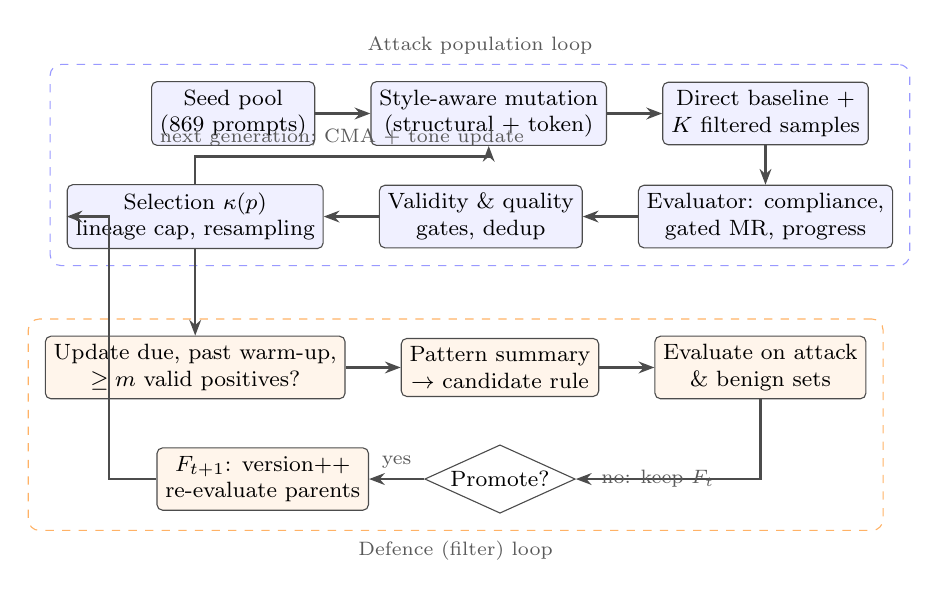
\begin{tikzpicture}[node distance=5mm and 7mm]
\node[attack] (seed) {Seed pool\\(\seedPoolSize{} prompts)};
\node[attack, right=of seed] (mut) {Style-aware mutation\\(structural + token)};
\node[attack, right=of mut] (gen) {Direct baseline +\\$K$ filtered samples};
\node[attack, below=of gen] (score) {Evaluator: compliance,\\gated MR, progress};
\node[attack, left=of score] (gates) {Validity \& quality\\gates, dedup};
\node[attack, left=of gates] (sel) {Selection $\kappa(p)$\\lineage cap, resampling};
\draw[flow] (seed) -- (mut);
\draw[flow] (mut) -- (gen);
\draw[flow] (gen) -- (score);
\draw[flow] (score) -- (gates);
\draw[flow] (gates) -- (sel);
\draw[flow] (sel.north) -- ++(0,0.35) -| node[note, pos=0.25, above] {next generation; CMA + tone update} (mut.south);
\node[defend, below=11mm of sel] (trig) {Update due, past warm-up,\\$\geq m$ valid positives?};
\node[defend, right=of trig] (rule) {Pattern summary\\$\rightarrow$ candidate rule};
\node[defend, right=of rule] (eval) {Evaluate on attack\\\& benign sets};
\node[decision, below=6mm of rule] (prom) {Promote?};
\node[defend, left=of prom] (ver) {$F_{t+1}$: version++\\re-evaluate parents};
\draw[flow] (sel) -- (trig);
\draw[flow] (trig) -- (rule);
\draw[flow] (rule) -- (eval);
\draw[flow] (eval) |- (prom);
\draw[flow] (prom) -- node[note, above] {yes} (ver);
\draw[flow] (ver.west) -| ++(-0.6,0) |- (sel.west);
\node[note, right=2mm of prom] {no: keep $F_t$};
\begin{scope}[on background layer]
\node[draw=blue!40, dashed, rounded corners, fit=(seed)(gen)(score)(sel), inner sep=6pt,
      label={[note]north:Attack population loop}] {};
\node[draw=orange!60, dashed, rounded corners, fit=(trig)(eval)(prom)(ver), inner sep=6pt,
      label={[note]south:Defence (filter) loop}] {};
\end{scope}
\end{tikzpicture}
\caption{Architecture of the coevolutionary testing framework. The attack loop (top) and the defence loop (bottom) share the filter version, so scores produced under different filters are never compared.}
\label{fig:architecture}
\end{figure}

\subsection{Prompt representation and initial population}
Each prompt is stored as a validated triple $(\mathit{prefix}, \mathit{body}, \mathit{suffix})$ with an explicit style tag, serialised with balanced internal markers (Figure~\ref{fig:mutation}). The representation lets a structural mutation \emph{replace} an existing frame instead of stacking frames, and it rejects malformed or leaked markers before any model call. An individual also stores its direct and filtered responses, metrics, filter version, and lineage identifiers: seed, parent, generation, and mutation log. Mutation clears all evaluation state, so a child can never inherit a parent's responses or fitness.

\subsection{Style directions and tone adaptation}
The study uses two tones, \emph{imperative} and \emph{plea}. They represent contrasting pragmatic pressure: command-like authority on one side and request-like emotional appeal on the other. For each tone $j$, a style direction is computed from positive and neutral anchor sets $S_j^+$, $S_j^0$ in a sentence-embedding space $E$ \citep{reimers2019sbert}:
\begin{equation}
d_j=\frac{\bar E(S_j^+)-\bar E(S_j^0)}{\|\bar E(S_j^+)-\bar E(S_j^0)\|_2+\epsilon}.
\end{equation}
Tones are chosen from a categorical distribution $\mathbf q_g$ rather than from the sign of a continuous control, so the mechanism extends to any number of tones. After selection at generation $g$, let $n_j$ be the number of surviving new offspring produced with tone $j$ and $n=\sum_j n_j$. The update is
\begin{equation}
q_{g+1}(j) \propto \max\!\Big(\varepsilon,\; (1-\eta)\,q_g(j) + \eta\,\tfrac{n_j}{n}\Big),
\end{equation}
with learning rate $\eta=0.2$ and floor $\varepsilon=0.02$, so that no tone disappears. The prototype sets and templates are versioned design elements. We do not claim they are psychological categories.

\begin{figure}[t]
\centering
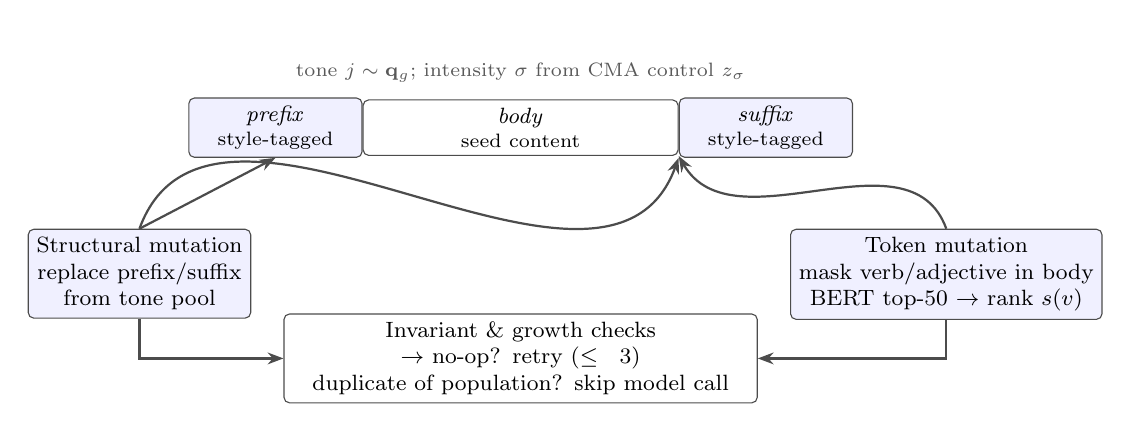
\begin{tikzpicture}[node distance=4mm and 6mm]
\node[box, minimum width=22mm, fill=blue!6] (pre) {\textit{prefix}\\[-1pt]{\scriptsize style-tagged}};
\node[box, minimum width=40mm, right=0mm of pre] (body) {\textit{body}\\[-1pt]{\scriptsize seed content}};
\node[box, minimum width=22mm, right=0mm of body, fill=blue!6] (suf) {\textit{suffix}\\[-1pt]{\scriptsize style-tagged}};
\node[attack, below left=9mm and -8mm of pre] (struct) {Structural mutation\\replace prefix/suffix\\from tone pool};
\node[attack, below right=9mm and -8mm of suf] (tok) {Token mutation\\mask verb/adjective in body\\BERT top-50 $\rightarrow$ rank $s(v)$};
\node[box, below=20mm of body, text width=58mm] (check) {Invariant \& growth checks $\rightarrow$ no-op? retry ($\leq 3$)\\duplicate of population? skip model call};
\draw[flow] (struct.north) -- (pre.south);
\draw[flow] (struct.north) to[out=70,in=-110] (suf.south west);
\draw[flow] (tok.north) to[out=110,in=-60] (body.south east);
\draw[flow] (struct.south) |- (check.west);
\draw[flow] (tok.south) |- (check.east);
\node[note, above=1mm of body] {tone $j\sim\mathbf q_g$; intensity $\sigma$ from CMA control $z_\sigma$};
\end{tikzpicture}
\caption{Internal prompt representation and the two mutation operators. Structural edits replace the style-tagged frame; token edits change one body token under a semantic-similarity constraint.}
\label{fig:mutation}
\end{figure}

\subsection{Structural and token mutation}
Structural mutation adds or replaces a style-tagged prefix or suffix drawn from the tone's template pool. Growth is bounded in absolute characters, relative to the seed body in characters and tokens, and by repeated $n$-grams and imperative fragments. Token mutation targets the body. A verb or adjective (or, as a fallback, an alphabetic span) is masked, BERT proposes 50 candidates \citep{devlin2019bert}, and each candidate $v$ replacing the original token $w$ is ranked by
\begin{equation}
s(v)=0.6\,e(v)^{\top}d_j+0.4\cos\big(e(v),e(w)\big),
\end{equation}
where candidates with $\cos(e(v),e(w))<0.5$ are discarded. The weighting is an implementation choice to be sensitivity-tested, not a claimed optimum. A child receives between one and $n_{\max}=2$ edits; the number grows with the mutation intensity $\sigma$. If all attempts are no-ops or rejected, up to three retries are made. An offspring whose rendered text exactly duplicates a population member is marked invalid without a model call.

\subsection{CMA-inspired Evolution Strategy}
Text is not optimised as a continuous vector. Instead, a control vector $z=(z_s,z_\sigma)\sim\mathcal N(\mathbf m,\eta_c^2\mathbf C)$ is sampled for each child \citep{hansen2016cma,beyer2002es}. The intensity is set as $\sigma=\mathrm{clip}(\sigma_0 e^{z_\sigma},\sigma_{\min},\sigma_{\max})$. The mean and the regularised covariance are re-estimated from the control vectors of the selected survivors. Survival is $(\mu+\lambda)$ by default. One-fifth-rule and self-adaptive variants are available for comparison. We call the method CMA-\emph{inspired} because the adaptation acts on mutation controls that are mapped to discrete operators.

\subsection{Diversity preservation and noise control}
Two mechanisms address failure modes observed in the pilot runs (Section~\ref{sec:diagnosis}).

\emph{Lineage cap.} During survivor selection, at most $c$ survivors may descend from the same seed prompt. Unfilled slots fall back to the best remaining candidates. This prevents one lucky lineage from taking every slot, which is the mechanism by which diversity collapsed in the pilot runs.

\emph{Parent resampling.} With plus-survival and $K\in\{2,3\}$, a parent with lucky samples keeps an inflated score indefinitely, a form of the winner's curse. Each surviving parent therefore receives $k_r$ fresh filtered samples per generation, up to $K_{\max}$ in total, and is re-scored on all of them.

Near-duplicate status is a relation between prompts, so it is recomputed at every ranking and the fitness each prompt had before being marked is restored. Section~\ref{sec:diagnosis} shows the cost of a persistent mark.

\subsection{Adaptive filter coevolution}
A filter update is attempted at generation $g$ only if three conditions hold: $g$ is a multiple of the update interval $u$, $g$ exceeds the warm-up $W$, and the ranked population contains at least $m$ distinct \emph{valid} prompts with $A>0$. The top-$k_f$ such prompts are summarised into broad defensive pattern classes (override, authority or role framing, urgency or plea framing, imperative pressure, obfuscation, fictional framing, procedural harm, cyber access, data exfiltration). The summaries are treated as inert data. An LLM proposes one additional rule, and pattern-specific fallback rules are tried if the proposal duplicates an existing rule or fails to improve safety. Let $S_A(F)$ be the attack-side safe rate (share of refusal plus benign educational responses), $R_B(F)$ the benign refusal rate, and $I(F)$ the invalid-response rate. A candidate $F'$ is eligible only if its invalid rates do not increase, and it is promoted if
\begin{equation}
\big[S_A(F')>S_A(F_t)\wedge R_B(F')\le R_B(F_t)+0.05\big]\;\vee\;\big[S_A(F')\ge S_A(F_t)\wedge R_B(F')<R_B(F_t)\big]. \label{eq:promotion}
\end{equation}
Figure~\ref{fig:promotion} summarises the procedure.

\begin{figure}[t]
\centering
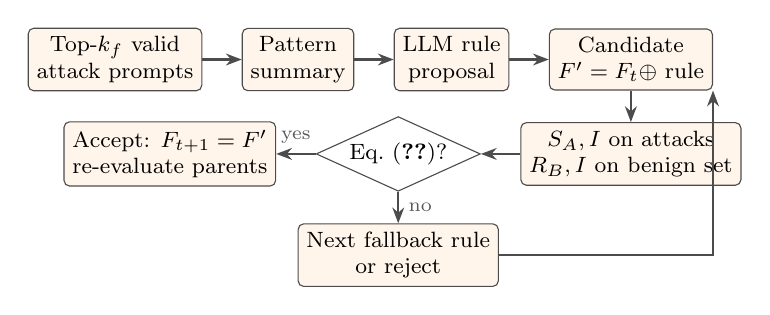
\begin{tikzpicture}[node distance=4mm and 5mm]
\node[defend] (top) {Top-$k_f$ valid\\attack prompts};
\node[defend, right=of top] (sum) {Pattern\\summary};
\node[defend, right=of sum] (prop) {LLM rule\\proposal};
\node[defend, right=of prop] (cand) {Candidate\\$F'=F_t\oplus$ rule};
\node[defend, below=of cand] (evalA) {$S_A,I$ on attacks\\$R_B,I$ on benign set};
\node[decision, left=of evalA] (crit) {Eq.~(\ref{eq:promotion})?};
\node[defend, left=of crit] (acc) {Accept: $F_{t+1}=F'$\\re-evaluate parents};
\node[defend, below=of crit] (fb) {Next fallback rule\\or reject};
\draw[flow] (top) -- (sum);
\draw[flow] (sum) -- (prop);
\draw[flow] (prop) -- (cand);
\draw[flow] (cand) -- (evalA);
\draw[flow] (evalA) -- (crit);
\draw[flow] (crit) -- node[note, above] {yes} (acc);
\draw[flow] (crit) -- node[note, right] {no} (fb);
\draw[flow] (fb.east) -| (cand.south east);
\end{tikzpicture}
\caption{Guardrailed filter promotion. A rule is accepted only if attack-side safety improves under a bounded benign-refusal cost (Eq.~\ref{eq:promotion}), or if safety is preserved while benign refusal decreases.}
\label{fig:promotion}
\end{figure}

\subsection{Filter-version consistency}
Changing the filter changes the fitness landscape, so every evaluation is tagged with its filter version. When a rule is accepted, active parents keep their direct baselines, lose their filtered outputs and fitness, and are re-evaluated under the new version before selection continues. Search-time and confirmation metrics are always reported separately.

\subsection{Defensive compliance evaluator}
The evaluator (\texttt{defensive-compliance-v5.3}) is deterministic and auditable. It detects refusals, defensive or educational content, operational harmful actionability, ambiguity, and invalid output. Harmful actionability overrides superficial disclaimers. Refused clauses are excluded from the harm scan, unless a continuation after a refusal is independently actionable. Numbered lists and the mere mention of a topic do not imply compliance. The evaluator is replaceable and is not treated as ground truth. Its calibration and its limits are reported in Section~\ref{sec:calibration}.

\subsection{Engineering pipeline for full-scale campaigns}
\label{sec:pipeline}
Full-scale campaigns require tens of thousands of model calls. The implementation therefore includes:
\begin{itemize}
\item concurrent model requests, including the benign and attack sets used in filter updates, with a deterministic record order;
\item artefacts streamed to disk after every generation (samples, generation history, filter events), which keeps memory flat and bounds data loss to one generation;
\item atomic checkpoints of the full search state (parents, CMA and tone state, filter, random-number-generator state), with resume and run extension guarded against configuration drift;
\item an explicit call-budget model (Section~\ref{sec:budget});
\item convergence analytics that re-score saved samples with the current evaluator.
\end{itemize}

\begin{algorithm}[t]
\caption{Coevolutionary prompt-injection search}
\label{alg:coevo}
\small
\begin{algorithmic}[1]
\Require seed pool $P_0$, filter $F_0$, generations $G$, parents $\mu$, offspring $\lambda$, update interval $u$, warm-up $W$
\State sample $\mu$ parents from $P_0$; evaluate them under $F_0$
\For{$g = 1,\dots,G$}
  \For{$i = 1,\dots,\lambda$}
    \State sample control $z\sim\mathcal N(\mathbf m,\eta_c^2\mathbf C)$ and tone $j\sim\mathbf q_g$; mutate a random parent (retry no-ops)
    \State \textbf{if} the child duplicates a population member \textbf{then} mark it invalid (no model call)
  \EndFor
  \State generate direct and $K$ filtered responses for the new offspring (concurrently); score and apply validity gates
  \State select $\mu$ survivors by $\kappa(p)$ with lineage cap $c$; update $(\mathbf m,\mathbf C)$ and $\mathbf q$
  \State resample surviving parents ($+k_r$ samples, up to $K_{\max}$) and re-score them
  \If{$g\bmod u=0$ \textbf{and} $g>W$ \textbf{and} at least $m$ valid positive prompts exist}
    \State propose a rule, evaluate $F'$ on the attack and benign sets
    \If{Eq.~\eqref{eq:promotion} holds}
      \State $F_{t+1}\gets F'$; invalidate filtered state; re-evaluate parents under $F_{t+1}$
    \EndIf
  \EndIf
  \State stream generation artefacts; checkpoint every $n_c$ generations
\EndFor
\State re-evaluate the final best prompt with $K_{\mathrm{conf}}$ fresh samples (out-of-search confirmation)
\end{algorithmic}
\end{algorithm}

%% ===========================================================================
\section{Experimental design}
\label{sec:design}

\subsection{Study structure}
The evaluation has three layers with distinct evidential roles, summarised in Table~\ref{tab:studies}. (i) A \emph{pilot series} of nine real-model runs, produced before the corrections of Section~\ref{sec:method}, is re-scored offline with the current evaluator and used for diagnosis (RQ4, RQ5). (ii) A \emph{simulated-target A/B study} checks that the corrections improve search on a calibrated landscape without spending model compute (RQ5). (iii) A \emph{full-scale real-model campaign} tests RQ1--RQ3 under paired seeds. Its results are marked \nm{} because the campaign has not yet been executed.

\begin{table}[t]
\centering
\caption{Evidence layers and their roles.}
\label{tab:studies}
\footnotesize
\begin{tabularx}{\linewidth}{@{}lXXl@{}}
\toprule
Layer & Purpose & Configuration & Status \\
\midrule
Pilot series & Diagnose search behaviour and filter dynamics on a real model & $\mu{=}8$, $\lambda{=}16$, $G{=}80$, $K{=}2$, $T{=}0.7$, scalar selection, behavioural deviation, update interval 5 (P1--P8) or fixed (P0) & completed; re-scored \\
Simulated A/B & Validate corrections on a calibrated landscape & $\mu{=}8$, $\lambda{=}32$, $G{=}60$, $K{=}2$, update interval 10, \abSeeds{} seeds & completed \\
Full-scale campaign & Answer RQ1--RQ3 with paired seeds & Table~\ref{tab:config} & \nm \\
\bottomrule
\end{tabularx}
\end{table}

\subsection{Target model and inference setting}
The target is a locally served LLM reached through an HTTP generation endpoint. The planned full-scale target is \texttt{dphn/Dolphin3.0-Llama3.1-8B}. Decoding uses at most 256 new tokens and $\text{top-}p=0.9$. Direct baselines are deterministic ($T=0$); filtered samples use $T=0.7$. The manifests of pilot runs P0--P4 record the model label \texttt{local-qwen} and those of P5--P8 the label \texttt{dolphin}. The client does not send this label to the server, so the checkpoint served during those runs cannot be verified from the artefacts. Model revision, quantisation, server software, and GPU for all layers: \nm.

\subsection{Datasets}
\paragraph{Seed pool} The initial population is sampled from \seedPoolSize{} labelled prompts (\texttt{prompts/initial\_population.csv}). This pool was drawn from a larger labelled corpus that appears to originate from the public \texttt{geekyrakshit/prompt-injection-dataset} \citep{geekyrakshit2024dataset}: 16 of 25 randomly probed seed prompts occur verbatim in that dataset. The derivation procedure and licence status still have to be confirmed [to be confirmed by the authors]. Table~\ref{tab:seedlabels} reports the structure and content labels. Harmful prompts are not reproduced in this paper.

\paragraph{Benign calibration and holdout sets} Filter promotion uses a fixed 40-prompt calibration set covering 13 categories. These include ordinary factual questions and benign security and incident-response requests, but also benign prompts written with imperative, urgent, or role-play framing, so that superficial style cues are penalised if they trigger refusal. A separate 12-prompt holdout set is evaluated only after search and never influences promotion.

\begin{table}[t]
\centering
\caption{Label distribution of the seed pool (one prompt may carry several labels).}
\label{tab:seedlabels}
\footnotesize
\begin{tabular}{@{}llr@{}}
\toprule
Kind & Label & Prompts \\
\midrule
Structure & \texttt{question\_request} & 534 \\
Structure & \texttt{imperative\_instruction} & 215 \\
Structure & \texttt{ignore\_all\_override} & 120 \\
Structure & \texttt{context\_wipe\_reset} & 1 \\
Structure & \texttt{forced\_start\_constraint} & 1 \\
Content & \texttt{hacking\_cybercrime} & 442 \\
Content & \texttt{violence} & 358 \\
Content & \texttt{bomb\_weapons} & 98 \\
Content & \texttt{policy\_bypass\_jailbreak} & 7 \\
Content & \texttt{child\_safety} & 4 \\
Content & \texttt{other\_illegal} & 3 \\
Content & \texttt{malware} & 2 \\
Content & \texttt{impersonation} & 2 \\
Content & \texttt{misinformation} & 1 \\

\bottomrule
\end{tabular}
\end{table}

\subsection{Conditions of the full-scale campaign}
Table~\ref{tab:conditions} lists the conditions. All share the seed list, the seed-pool hash, the budget, and the decoding policy. C1 and C2 form the central paired comparison (RQ3). C3 and C4 are ablations of the corrections, showing whether they improve real-model search (RQ5); C4 reproduces the legacy search controls, although the corrected quality gates cannot be switched off. C5 and C6 isolate the mutation operators (RQ2), and C0 is the unsearched baseline (RQ1).

\begin{table}[t]
\centering
\caption{Planned full-scale conditions. All use the settings of Table~\ref{tab:config} unless stated otherwise.}
\label{tab:conditions}
\footnotesize
\begin{tabularx}{\linewidth}{@{}llX@{}}
\toprule
ID & Filter & Change relative to C1 \\
\midrule
C0 & fixed & seed prompts evaluated without search (matched sample budget) \\
C1 & coevolution & none (proposed configuration) \\
C2 & fixed & filter updates disabled \\
C3 & coevolution & progress tie-breaker disabled \\
C4 & coevolution & legacy search controls: no retry, duplicates evaluated, no lineage cap, no resampling, uniform tones, no warm-up \\
C5 & fixed & structural mutation only \\
C6 & fixed & token mutation only \\
\bottomrule
\end{tabularx}
\end{table}

\subsection{Search configuration}
Table~\ref{tab:config} gives the configuration of the full-scale campaign (the \texttt{full} preset of the implementation).

\begin{table}[t]
\centering
\caption{Full-scale search configuration.}
\label{tab:config}
\footnotesize
\begin{tabular}{@{}ll@{}}
\toprule
Parameter & Value \\
\midrule
Optimiser & CMA-inspired ES, $(\mu+\lambda)$, $\sigma\in[0.25,6]$ \\
Parents $\mu$ / offspring $\lambda$ / generations $G$ & 16 / 64 / 300 \\
Filtered samples per prompt $K$ / confirmation $K_{\mathrm{conf}}$ & 3 / 16 \\
Parent resampling $k_r$ / cap $K_{\max}$ & 1 / 12 \\
Lineage cap $c$ & 4 \\
Tones / adaptation & imperative, plea / categorical ($\eta=0.2$, $\varepsilon=0.02$) \\
Mutation edits per child / no-op retries & $\leq 2$ / $\leq 3$ \\
Filter update interval $u$ / warm-up $W$ / min.\ positives $m$ / $k_f$ & 15 / 30 / 3 / 8 \\
Benign-refusal tolerance in Eq.~\eqref{eq:promotion} & 0.05 \\
Stagnation reporting window & 40 generations \\
Concurrent model requests / checkpoint interval & 8 / 5 generations \\
Seeds & 101, 202, 303 \\
\bottomrule
\end{tabular}
\end{table}

\subsection{Compute budget}
\label{sec:budget}
The number of model calls is estimated as
\begin{equation}
N \approx G\lambda(1-\rho)(1+K) + G\mu k_r + U\big[(|B|+k_f)(1+R)+1+\mu(1+K)\big] + K_{\mathrm{conf}}+1,
\end{equation}
where $\rho$ is the share of duplicate offspring, $U=\lfloor (G-W)/u\rfloor$ is the number of update attempts, $|B|$ is the benign set size, and $R$ is the mean number of candidate rules per update. With $\rho=0.05$, $R=4$, and $|B|=40$, the configuration of Table~\ref{tab:config} requires about \budgetCalls{} calls per run: \budgetSearchCalls{} for search, at most \budgetResampleCalls{} for resampling, and \budgetFilterCalls{} for filter updates. At 2.5\,s per call this is \budgetHoursSequential{}\,h sequentially, or about \budgetHours{}\,h with eight concurrent requests. The measured per-call latency of the campaign server is \nm.

\subsection{Outcome measures}
\paragraph{Primary} The confirmed attack objective of the final best prompt, re-evaluated with $K_{\mathrm{conf}}$ fresh samples, and the benign-holdout refusal rate of the final filter.

\paragraph{Search dynamics} Let $c_g$ be the share of offspring filtered samples labelled compliant at generation $g$ and $\bar c_g$ its 5-generation trailing mean. We report the first generation with $c_g>0$; the convergence times $t_\alpha=\min\{g:\bar c_g\geq\alpha\max_h\bar c_h\}$ for $\alpha\in\{0.5,0.9\}$; the longest stretch without a new best $\bar c$; and \emph{critical improvement points}, defined as the largest single-generation rises of $\max_{h\le g}\bar c_h$ that each exceed 10\% of the peak.

\paragraph{Filter dynamics} For every accepted update at generation $g_u$, we compare the mean $c$ over the five generations up to $g_u$ with the mean over the five generations after it, and record the half-recovery time, the first $g>g_u$ with $\bar c_g$ at or above half the pre-update mean.

\paragraph{Diagnostics} We record the invalid share of parent slots by gate, the no-op share of mutation attempts, population diversity (mean pairwise Jaccard token distance), the number of surviving seed lineages, the tone probabilities, and the lead correlation between non-compliant progress $\Pi-c$ at generation $g$ and compliance $c_{g+3}$.

\subsection{Statistical analysis}
Fixed-filter and coevolution runs with the same seed are paired. For each primary contrast we will report per-seed paired differences, their mean with a 95\% confidence interval, and the paired effect size. With three seeds, significance tests have little power, so intervals and raw paired differences are emphasised. Wilcoxon signed-rank tests are reported only as a robustness check, and contrasts within one hypothesis family receive a Holm correction. Convergence curves show per-seed trajectories.

\subsection{Simulated target}
\label{sec:simulator}
The simulated target returns only fixed, sanitised template responses, one per evaluator class, and no model text. A hidden susceptibility score is computed for each filtered request:
\begin{equation}
z = 0.55\min\!\big(6,|\mathcal W(p)\cap\mathcal L|\big) + u(p) - 0.35\,r(F) + \sum_j \mathbb 1_j(p)\big(\beta_j - 1.2\,\mathbb 1_j(F)\big) + \epsilon,
\end{equation}
where $\mathcal L$ is a hidden lexicon of 30 ordinary words, $u(p)$ is a fixed per-prompt offset in $[-0.75,0.75]$, $r(F)$ is the number of filter rules, $\beta_{\text{plea}}=0.9$, $\beta_{\text{imp}}=0.4$, $\mathbb 1_j(F)$ indicates a rule that names tone $j$, and $\epsilon\sim\mathcal N(0,0.6^2)$ applies when $T>0$. The response is compliant with probability $\sigma(z-d)$, where $d=\simDifficulty{}$, which gives a seed-pool base rate of \simBaseRate{} and so matches the sparsity of the real model. Otherwise, the probability of an ambiguous or educational response rather than a refusal rises with $z$. This monotone relation between openness and compliance is exactly the assumption that the progress tie-breaker relies on, so simulator results validate mechanics and relative settings, not real-model behaviour. Benign requests are refused with a probability that grows by 0.02 per filter rule.

%% ===========================================================================
\section{Results}
\label{sec:results}

\subsection{Evaluator calibration}
\label{sec:calibration}
On the committed calibration fixture, the evaluator labels \calibCorrect{} of \calibTotal{} sanitised responses correctly (Table~\ref{tab:calibration}). The fixture is small and was built together with the evaluator, so this establishes internal consistency, not accuracy. Agreement with human annotation on a sample of real responses: \nm. One observation qualifies later compliance figures. In one pilot run, the single most frequent operational pattern accounts for up to \pilotTopPatternShareMax{} of all compliant labels, so compliance counts are sensitive to the coverage of individual rules.

\begin{table}[t]
\centering
\caption{Confusion matrix of the evaluator on the calibration fixture (rows: expected label; columns: predicted label).}
\label{tab:calibration}
\footnotesize
\begin{tabular}{@{}lccccc@{}}
\toprule
 & refusal & benign\_edu. & compliant & ambiguous & invalid \\
\midrule
\texttt{refusal} & 7 & 0 & 0 & 0 & 0 \\
\texttt{benign\_educational} & 0 & 2 & 0 & 0 & 0 \\
\texttt{compliant} & 0 & 0 & 6 & 0 & 0 \\
\texttt{ambiguous} & 0 & 0 & 0 & 1 & 0 \\
\texttt{invalid} & 0 & 0 & 0 & 0 & 1 \\

\bottomrule
\end{tabular}
\end{table}

\subsection{Pilot series on a real model}
\label{sec:pilot}
Table~\ref{tab:pilot} summarises the nine pilot runs after re-scoring. Across \pilotSamples{} filtered responses, \pilotShareRefusal{} were refusals, \pilotShareBenign{} benign educational, \pilotShareAmbiguous{} ambiguous, and \pilotShareCompliant{} compliant. Compliance is concentrated in a few runs (P4, P5, P7). The fixed-filter run P0 remains near 0.007 throughout, whereas coevolution run P7 rises to 0.404 in its last quarter (Figure~\ref{fig:pilot}). These runs differ in software version as well as filter mode, so they do not form a controlled comparison. They are reported as diagnostic evidence, and RQ1 and RQ3 are left to the full-scale campaign.

\begin{table}[t]
\centering
\caption{Pilot series (re-scored with the current evaluator). Rate = share of filtered samples labelled compliant; $t_{90}$ = first generation at 90\% of the smoothed peak; ND and Other = mean invalid share of parent slots due to near-duplicate marks and to other gates; Div.\ = population diversity at the first and last generation. $^\dagger$Runs quarantined in the repository registry for diagnostic use only.}
\label{tab:pilot}
\scriptsize
\setlength{\tabcolsep}{3pt}
\begin{tabular}{@{}llrrrrrrrrrrl@{}}
\toprule
Run & Model label & $u$ & Upd. & Samples & Rate & Early & Late & First & $t_{90}$ & ND & Other & Div. \\
\midrule
P0 (fixed) & local-qwen & 0 & 0 & 2560 & 0.007 & 0.006 & 0.008 & 9 & 12 & 0.73 & 0.00 & 0.93$\to$0.93 \\
P1 & local-qwen & 5 & 1 & 2576 & 0.049 & 0.073 & 0.041 & 1 & 2 & 0.92 & 0.00 & 0.91$\to$0.52 \\
P2 & local-qwen & 5 & 3 & 2608 & 0.003 & 0.002 & 0.003 & 7 & 7 & 0.84 & 0.00 & 0.94$\to$0.31 \\
P3 & local-qwen & 5 & 1 & 2576 & 0.007 & 0.019 & 0.006 & 1 & 1 & 0.58 & 0.00 & 0.93$\to$0.70 \\
P4 & local-qwen & 5 & 2 & 2592 & 0.465 & 0.445 & 0.467 & 1 & 7 & 0.82 & 0.00 & 0.91$\to$0.43 \\
P5 & Dolphin & 5 & 8 & 2688 & 0.141 & 0.148 & 0.141 & 1 & 17 & 0.82 & 0.18 & 0.94$\to$0.15 \\
P6$^{\dagger}$ & Dolphin & 5 & 6 & 2656 & 0.019 & 0.005 & 0.017 & 14 & 43 & 0.74 & 0.00 & 0.93$\to$0.28 \\
P7 & Dolphin & 5 & 8 & 2688 & 0.232 & 0.121 & 0.404 & 1 & 72 & 0.80 & 0.14 & 0.92$\to$0.24 \\
P8$^{\dagger}$ & Dolphin & 5 & 8 & 2688 & 0.011 & 0.021 & 0.006 & 1 & 12 & 0.84 & 0.15 & 0.92$\to$0.15 \\

\bottomrule
\end{tabular}
\end{table}

\begin{figure}[t]
\centering
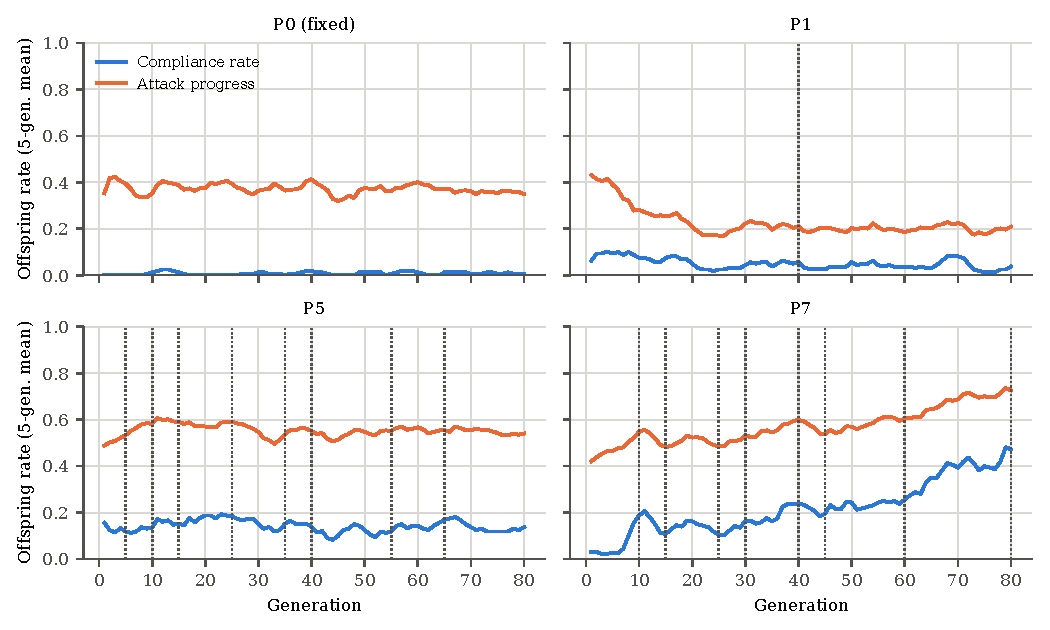
\includegraphics[width=\linewidth]{figures/pilot_curves.pdf}
\caption{Re-scored offspring compliance rate and attack progress (5-generation trailing means) for four pilot runs. Dotted lines mark accepted filter updates.}
\label{fig:pilot}
\end{figure}

\subsection{Diagnosis of search starvation (RQ5)}
\label{sec:diagnosis}
Three implementation faults explain why fitness was often zero from the first generations.

\emph{Garbled-token gate.} The legacy gate flagged a token as garbled when its letter bigrams fell outside a list of about 50 common pairs. Ordinary words such as ``explain'' failed this test. Under the legacy gates only \seedValidLegacy{} of \seedPoolSize{} seed prompts were valid, and \seedGarbledLegacy{} (\seedGarbledLegacyPct{}) were rejected as garbled before any mutation. The corrected rules flag only character shapes that machine-garbled tokens have and real words and deliberate typo obfuscations do not (digit--letter mixes, runs of the same character, long vowel-free or consonant-only runs, over-long tokens). Under them \seedValidCurrent{} of \seedPoolSize{} seeds are valid.

\emph{Persistent near-duplicate marks.} Once a parent had been marked as a near duplicate, it kept zero fitness even after the prompt it duplicated had left the population. Figure~\ref{fig:gates} shows that near-duplicate marks invalidated \pilotNearDupMin{}--\pilotNearDupMax{} of parent slots on average. In P5 and P8, the other gates bring the combined invalid share to 0.99--1.00, which is essentially the whole population. Selection then operated among one or two effective candidates.

\emph{No-op mutations.} \pilotNoopMin{}--\pilotNoopMax{} of mutation attempts changed nothing. The resulting copies were still sent to the model and then discarded as duplicates.

\begin{figure}[t]
\centering
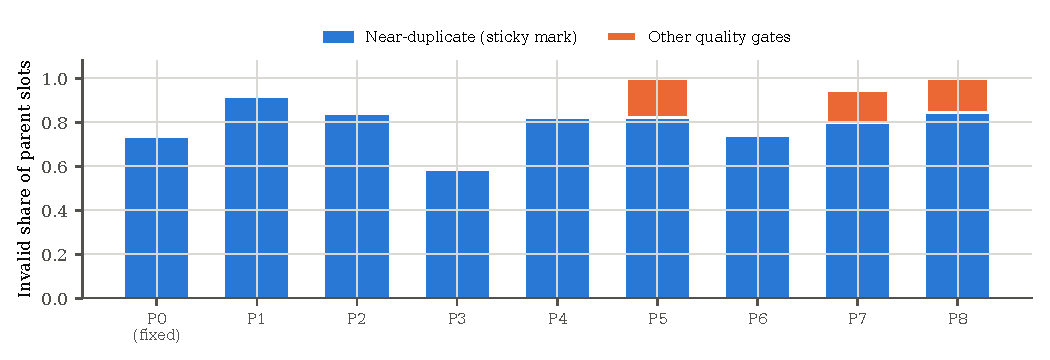
\includegraphics[width=\linewidth]{figures/gate_losses.pdf}
\caption{Mean share of parent slots invalidated by the persistent near-duplicate mark and by other quality gates in the pilot series.}
\label{fig:gates}
\end{figure}

\subsection{Filter-update dynamics (RQ4)}
The pilot series contains \shockCount{} accepted filter updates. Aligned on the update generation (Figure~\ref{fig:events}), the offspring compliance rate shows no measurable immediate suppression: the median pre-to-post drop is \shockMedianDrop{}, and in \shockRecoveredWithinOne{} of the \shockRecoverable{} updates with non-zero pre-update compliance, the rate returned to half its prior level within one generation. With updates every five generations, promoted rules were therefore either too specific to affect the next offspring or were circumvented immediately. Together with the diagnosis above, this indicates that the early zero-fitness plateaus were caused mainly by search bookkeeping rather than by the defence. This motivated the warm-up and minimum-evidence triggers.

\begin{figure}[t]
\centering
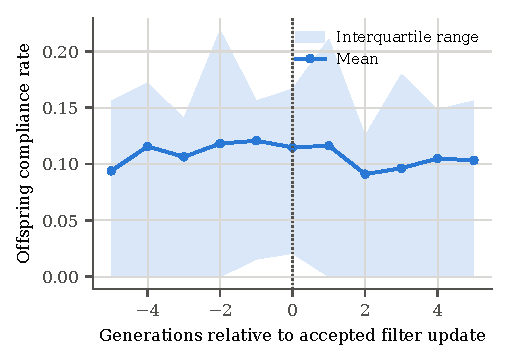
\includegraphics[width=0.6\linewidth]{figures/filter_events.pdf}
\caption{Offspring compliance rate aligned on accepted filter updates in the pilot series (mean and interquartile range over events).}
\label{fig:events}
\end{figure}

\subsection{Validity of the progress signal}
Progress and compliance are correlated within a generation (median Pearson $r=\progressSameMedian{}$ over the pilot runs). The component of progress that excludes compliance, however, does not predict compliance three generations later: the median lead correlation is \progressLeadMedian{}, positive in \progressLeadPositive{} of \progressLeadCount{} runs. In this real-model data, therefore, there is no evidence that non-compliant progress is a stepping stone towards compliance. Because progress only breaks ties below the true objective, the cost of this uncertainty is bounded, and condition C3 of the full-scale campaign tests it directly.

\subsection{Simulated-target validation of the corrections (RQ5)}
Table~\ref{tab:ab} and Figure~\ref{fig:ab} compare the legacy search controls with the proposed ones on the simulated target. The corrected quality gates are active in both arms, so the comparison isolates the search controls. The proposed controls raise the mean offspring success rate from \abLegacyMeanSuccess{} to \abImprovedMeanSuccess{} (\abRelativeGain{} relative) and are higher in all \abSeeds{} seeds. Population diversity stays near \abImprovedDiversity{} instead of collapsing to \abLegacyDiversity{}, and \abImprovedLineages{} seed lineages survive instead of \abLegacyLineages{}, while using slightly fewer model calls (\abImprovedCalls{} versus \abLegacyCalls{}). Two results do not favour the proposed controls. The number of generations with zero best fitness is lower in only one seed, and the highest fitness ever observed is lower (Table~\ref{tab:ab}). The second result is consistent with parent resampling removing lucky high estimates, but that explanation has not been tested. Because the simulator encodes the progress assumption, these gains are an upper bound on what the progress component can contribute on a real model.

\begin{table}[t]
\centering
\caption{Simulated-target A/B (means over \abSeeds{} seeds). The last column counts seeds in which the proposed value exceeds the legacy value; for model calls and zero-fitness generations, lower is better.}
\label{tab:ab}
\footnotesize
\begin{tabular}{@{}lrrc@{}}
\toprule
Metric & Legacy & Proposed & Proposed $>$ legacy \\
\midrule
Mean offspring success rate & 0.026 & 0.039 & 3/3 \\
Early-quarter offspring success rate & 0.063 & 0.074 & 2/3 \\
Late-quarter offspring success rate & 0.010 & 0.012 & 3/3 \\
Late-quarter offspring progress & 0.013 & 0.021 & 3/3 \\
Generations with best fitness $=0$ & 15.0 & 9.3 & 1/3 \\
Surviving seed lineages (final) & 1.0 & 4.0 & 3/3 \\
Population diversity (final) & 0.40 & 0.79 & 3/3 \\
Best fitness ever observed & 0.846 & 0.720 & 1/3 \\
Model calls & 5819 & 5620 & 0/3 \\
Accepted filter updates & 3.7 & 3.0 & 0/3 \\

\bottomrule
\end{tabular}
\end{table}

\begin{figure}[t]
\centering
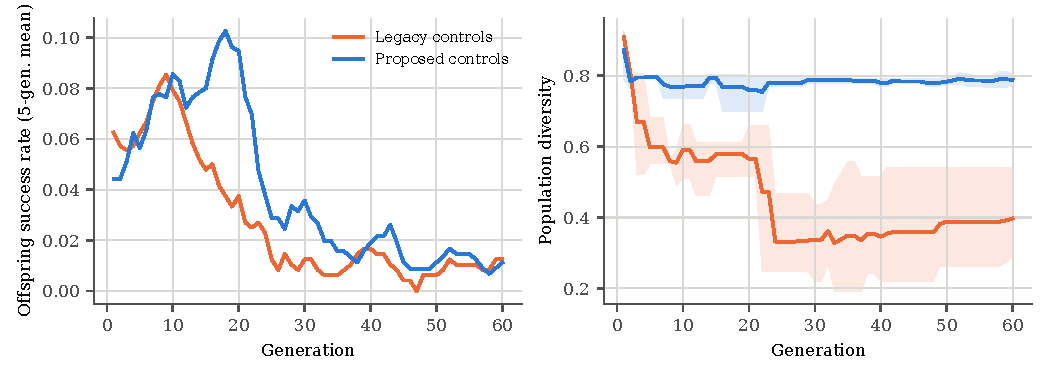
\includegraphics[width=\linewidth]{figures/simulated_ab.pdf}
\caption{Simulated-target A/B. Left: offspring success rate (seed mean, 5-generation trailing mean). Right: population diversity (seed mean and range).}
\label{fig:ab}
\end{figure}

\subsection{Full-scale campaign (RQ1--RQ3)}
The full-scale campaign of Table~\ref{tab:conditions} has not yet been executed. Tables~\ref{tab:rq1}--\ref{tab:confirm} fix the reporting format; each value will be taken directly from the run manifests and the analysis scripts.

\begin{table}[t]
\centering
\caption{RQ1 and RQ2: search effectiveness under a fixed filter (per-seed mean $\pm$ s.d.).}
\label{tab:rq1}
\footnotesize
\begin{tabular}{@{}lcccc@{}}
\toprule
Condition & Confirmed $A$ & Fluency & Diversity & $t_{90}$ \\
\midrule
C0 seed, no search & \nm & \nm & \nm & -- \\
C2 full search, fixed filter & \nm & \nm & \nm & \nm \\
C5 structural only & \nm & \nm & \nm & \nm \\
C6 token only & \nm & \nm & \nm & \nm \\
\bottomrule
\end{tabular}
\end{table}

\begin{table}[t]
\centering
\caption{RQ3: paired fixed-filter and coevolution comparison.}
\label{tab:rq3}
\footnotesize
\begin{tabular}{@{}lccccc@{}}
\toprule
Condition & Confirmed $A$ & $S_A$ & Benign refusal (holdout) & Updates accepted & Filter length \\
\midrule
C2 fixed & \nm & \nm & \nm & 0 & \nm \\
C1 coevolution & \nm & \nm & \nm & \nm & \nm \\
Paired difference (95\% CI) & \nm & \nm & \nm & -- & \nm \\
\bottomrule
\end{tabular}
\end{table}

\begin{table}[t]
\centering
\caption{Search-time versus out-of-search confirmation of the selected prompts (C1).}
\label{tab:confirm}
\footnotesize
\begin{tabular}{@{}lccc@{}}
\toprule
Metric & Search & Confirmation & Difference \\
\midrule
Attack objective $A$ & \nm & \nm & \nm \\
MR & \nm & \nm & \nm \\
Fitness $f$ & \nm & \nm & \nm \\
Samples & \nm & 16 & -- \\
\bottomrule
\end{tabular}
\end{table}

%% ===========================================================================
\section{Discussion}
\label{sec:discussion}

\subsection{Interpreting adaptive attack search}
The compliance-primary design separates genuine attack improvement from movement in secondary metrics. A prompt that grows longer, drifts semantically, or diverges from its direct response without producing harmful compliance is not a stronger injection. The pilot series shows why confirmation matters. Rates in the same budget class range from below 0.01 to 0.47, and much of that spread plausibly reflects evaluator coverage and implementation state rather than search quality. Claims about RQ1 will therefore rest on confirmed, out-of-search responses and on the paired design.

\subsection{Interpreting style effects}
Imperative and plea tones are controlled linguistic directions, not models of users. With categorical adaptation, the tone probabilities themselves become an outcome: a tone whose probability rises after a filter update indicates that the model and filter are sensitive to that framing. Structural frames also add length, so tone effects must be checked against prompt-length and seed-growth statistics before they are attributed to style.

\subsection{Interpreting filter coevolution}
The promotion criteria (Eq.~\ref{eq:promotion}) keep the defence from buying attack-side safety with indiscriminate refusal, and the independent holdout provides a stronger check after search. In the pilot series, promoted rules did not measurably reduce offspring compliance. If the full-scale campaign shows the same, one explanation is that a single appended rule cannot counter a broad style shift. Another is that the attack population recovers within a generation, which is an arms-race dynamic that static evaluation would miss. Both outcomes are informative for defence engineering.

\subsection{Measurement hygiene in evolutionary LLM testing}
In our pilot data, the most consequential failures were silent. Two quality gates, each plausible in isolation, invalidated almost the whole population and made zero fitness look like defensive strength. Three practices would have exposed them: auditing the gates on the unmutated seed pool, reporting invalid shares by reason for every generation, and tracking offspring-level rather than elite-level metrics. Under plus-survival, elite metrics plateau even when the search has stopped producing anything. We recommend these audits as standard reporting for evolutionary red-teaming studies.

\subsection{Engineering implications}
For practitioners, the framework is a budgeted test harness. The call-budget model turns a test plan into hours of inference. Checkpoints make multi-day campaigns robust to server failures. Streaming the per-generation analytics allows a campaign to be stopped early once $t_{90}$ has been reached. The filter under test can be replaced by an embedding detector, an architectural isolation layer, or a model-level defence while keeping the attack population, the promotion criteria, and the version semantics.

\subsection{Limitations}
\emph{Single model and missing campaign.} All real-model evidence comes from pilot runs whose served checkpoint cannot be verified from the artefacts, and the full-scale results are \nm.
\emph{Evaluator.} The rule-based evaluator is auditable but incomplete. Its calibration fixture is small, compliance counts depend on the coverage of individual patterns, and human-audit agreement is \nm.
\emph{Progress signal.} The progress tie-breaker has no demonstrated predictive value on the real model, and its benefit in simulation is partly built into the simulator.
\emph{Style space.} Only two tones are studied. The adaptation mechanism supports more, but other framings are not evaluated.
\emph{CMA terminology.} Adaptation acts on mutation controls, not on text, so the theory of continuous CMA-ES does not transfer.
\emph{Data.} The provenance and licence of the seed pool are still to be confirmed, the benign sets are small, and all prompts are in English.
\emph{Stochasticity and budget.} Three seeds and $K\le 3$ leave substantial noise, and final confirmation reduces but does not remove the winner's curse.
\emph{Defence overfitting.} A coevolved filter may overfit the current attack population. Attack-family holdouts and cross-run transfer tests are needed.

\subsection{Ethical and safety considerations}
The framework is intended for defensive measurement. Fixtures, references, and simulator responses are sanitised and non-operational. Raw model outputs from real runs may contain sensitive text; they are kept out of public releases unless reviewed, and this paper reports only aggregate metrics. Attack examples passed to the filter-updating model are marked as inert data. Credentials are supplied through environment variables and redacted from artefacts. Experiments are run only on locally hosted models that the authors are authorised to use; no external systems or third-party services are targeted.

%% ===========================================================================
\section{Conclusion}
\label{sec:conclusion}
We presented a coevolutionary framework that tests prompt-level LLM defences against an adaptive, style-aware evolutionary attacker. Filter adaptation is guarded by measurable promotion criteria and strict version semantics. Re-scoring real-model pilot runs showed that search efficiency was limited mainly by implementation-level quality gates rather than by the defence: the legacy gates invalidated \seedGarbledLegacyPct{} of the seed prompts, and persistent duplicate marks invalidated most parent slots. We corrected these faults and added a search-only progress tie-breaker, a lineage cap, parent resampling, categorical tone adaptation, and filter warm-up. On a calibrated simulated target, the mean offspring success rate improved by \abRelativeGain{} and population diversity was preserved. The pipeline is concurrent, checkpointed, and budgeted for full-scale campaigns, and the paired full-scale real-model study (RQ1--RQ3) is the next step. Future work will extend the framework to more models, tones, and languages, to learned response evaluators audited against human labels, and to held-out attack families.

%% ===========================================================================
\section*{CRediT authorship contribution statement}
[To be completed by the authors using CRediT roles that reflect actual contributions.]

\section*{Declaration of competing interest}
[To be completed with the Elsevier-required statement.]

\section*{Funding}
This work was supported by the Scientific and Technological Research Council of T\"urkiye (T\"UB\.ITAK) under the 1002-A programme, project number [project number].

\section*{Data availability}
Code, analysis scripts, aggregate run summaries, the calibration fixture, and the benign sets will be released at [repository/DOI]. Raw model generations, which may contain sensitive text, are not released by default. The seed pool is derived from a public dataset \citep{geekyrakshit2024dataset}, subject to confirmation of its licence.

\section*{Declaration of generative AI and AI-assisted technologies in the writing process}
[To be completed by the authors. It must accurately describe any AI assistance used in preparing the manuscript, the code, or the analyses, and the authors remain responsible for the content.]

%% References not cited in the text are listed at the end.
\nocite{*}
\bibliographystyle{elsarticle-harv}
\bibliography{refs}

\end{document}
